\newpage
\section{Michał Dul}
\label{sec:dulmicha}

\subsection{Humans' best friends}
The Labrador Retriever, often abbreviated to \emph{Labrador} or \emph{"Lab"}, is a breed of retriever gun dog from the United Kingdom that was developed from imported Canadian fishing dogs. \textbf{The Labrador is one of the most popular dog breeds in a number of countries in the world}, particularly in the Western world.

\begin{figure}[H]
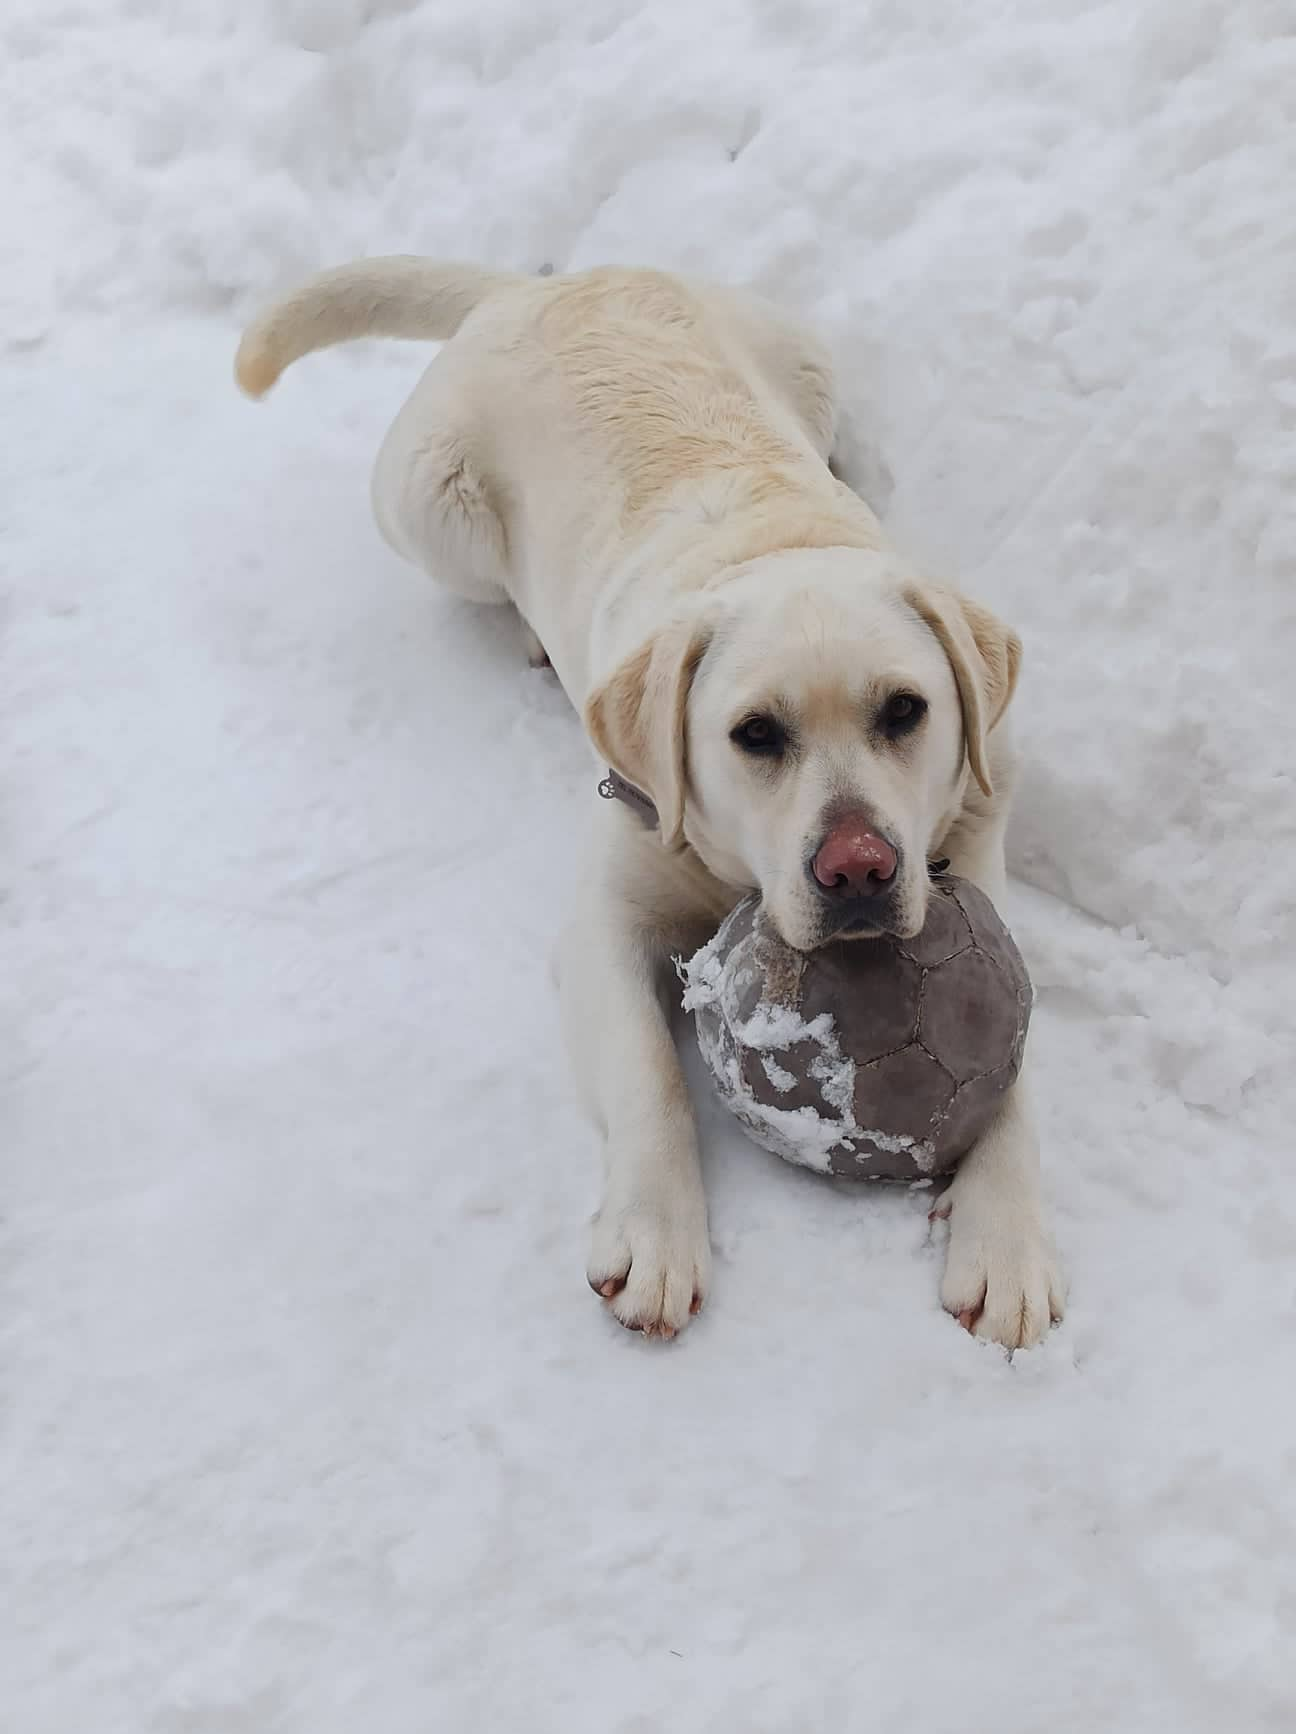
\includegraphics[scale=0.1]{pictures/dulmicha/tobi.jpg}
\centering
\caption{Labrador Retriever}
\label{fig:tobi}
\end{figure}

A popular disability assistance breed in many countries, Labradors are frequently trained to aid those with blindness or autism, act as a therapy dog, or perform screening and detection work for law enforcement and other official agencies. The breed is best known for their \underline{obedience}, \underline{loyalty}, and \underline{playful composure}. Additionally, they are prized as sporting and hunting dogs. Ancestors include a breed used in Newfoundland as fishing dogs, that would help in bringing in the fishing nets and recapture escaped fish.

\subsection{Acceptable Labs colours}
\begin{itemize}
    \item[--] chocolate 
    \item[--] yellow
    \item[--] black
\end{itemize}

\subsection{Get to know them better!}
When they compared the dog DNA data to information from humans, the researchers came up with a new equation to figure out the dog's comparable human age. The equation: 
\[16ln(dogage) + 31 = humanage.\]

In fact, doggos size also matters, as shown down there:
\begin{table}[H]
\caption{Dog-to-human age referred to weight}
\label{table:doggos_years}
\tiny
\centering
\resizebox{\textwidth}{!}{%
\begin{tabular}{
>{\columncolor[HTML]{FFCC67}}l 
>{\columncolor[HTML]{FFFFC7}}l 
>{\columncolor[HTML]{FFFFC7}}l 
>{\columncolor[HTML]{FFFFC7}}l 
>{\columncolor[HTML]{FFFFC7}}l }
Size of dog & \cellcolor[HTML]{FFCC67}Small & \cellcolor[HTML]{FFCC67}Medium & \cellcolor[HTML]{FFCC67}Large & \cellcolor[HTML]{FFCC67}Giant \\
Age of dog & \multicolumn{4}{l}{\cellcolor[HTML]{FFCE93}Age in human years} \\
1 year & 15 & 15 & 15 & 15 \\
2 & 24 & 24 & 24 & 22 \\
3 & 28 & 28 & 28 & 31 \\
4 & 32 & 32 & 32 & 38 \\
5 & 36 & 36 & 36 & 45 \\
6 & 40 & 42 & 45 & 49 \\
7 & 44 & 47 & 50 & 56 \\
8 & 48 & 51 & 55 & 64 \\
9 & 52 & 56 & 61 & 71 \\
10 & 56 & 60 & 66 & 79 \\
11 & 60 & 65 & 72 & 86 \\
12 & 64 & 69 & 77 & 93 \\
13 & 68 & 74 & 82 & 100 \\
14 & 72 & 78 & 88 & 107 \\
15 & 76 & 83 & 93 & 114
\end{tabular}%
}
\end{table}

Table~\ref{table:doggos_years} implicates that Labradors (example: photo~\ref{fig:tobi}) live shorter than other, smaller breeds. 

\subsection{Trick or treat?}
The most popular dog tricks:
\begin{enumerate}
  \item Bark on command
  \item Shake hands
  \item Roll over
  \item Play dead
\end{enumerate}